\subsection{Umfrage-Dashboard}
\label{ssec:UmfrageDashboard}

Wie zuvor in Kapitel \myRefGeneral{ssec:UmfrageErstellen} dargestellt, ist das Herzstück der Applikation das Erstellen einer Umfrage.
Nachdem der Benutzer eine Umfrage \engl{Survey} angelegt hat, findet dieser die Umfrage auf der hier vorgestellten Seite wieder.

Abbildung~\myRefGeneral{fig:SurveyMasterDashboard} zeigt das \emph{Survey Dashboard}.
Der Benutzer kann hier über ein Suchleiste, die auch als Dropdown-Menü fungiert, seine erstellten Umfragen nach Namen filtern. \newline
Die erste Karte auf dieser Seite ist von ihrem Aufbau her differenziert.
Über den Knopf \jinline|Create New Survey Master| auf der Karte mit dem Icon \faPlusSquare, kann der Benutzer eine neue Umfragevorlage \emph{(Survey Master)} anlegen (siehe Kapitel~\vref{ssec:UmfrageErstellen}). \newline
Die anderen Karten folgen einem gleichen Muster:
%
\begin{itemize}
	\item Sie beinhalten immer die Anzahl der erstellten (published) Umfragen.
	\item Eine Survey kann immer über das Icon \faCopy\xspace kopiert werden.
	Hierbei werden alle Fragen übernommen und die Umfrage kann optional verändert werden.
\end{itemize}
%
Generell unterscheiden sich die Umfragen wie folgt:
%
\subsubsection*{Survey-Template -- keine Umfrage erstellt}
%
Der Benutzer hat die Möglichkeit, im Falle einer Falscheingabe über das Icon \faEdit\xspace wieder in den Editierungsmodus zu gelangen (vgl. Abschnitt~\vref{ssec:UmfrageErstellen}).
Dadurch wird Anforderung~\hyperref[Anf:A11]{A11}, die Bearbeitbarkeit unveröffentlichter Umfragen, erfüllt.
Über das Icon \faTrash\xspace lässt sich die erstellte Umfrage wieder löschen, da es hierzu noch keine gestartete Umfrage gibt.

\subsubsection*{Survey-Template -- mindestens eine Umfrage ist erstellt}
%
Da die Umfrage bereits gestartet ist, entfallen nun die Icons \faTrash\xspace (löschen) und \faEdit\xspace (editieren).
Als ein Alleinstellungsmerkmal hat der Benutzer nun die Möglichkeit über das Icon \faIdCard\xspace zu seinen Ergebnissen zu kommen (vgl. Abschnitt~\vref{ssec:ResultDashboardImplement}).

Dadurch wird Anforderung~\hyperref[Anf:A8]{A8}, das Verwalten von Umfragen, sowie die Anforderung~\hyperref[Anf:A12]{A12}, die Wiederholbarkeit von Umfragen, erfüllt.

\begin{figure}[!htb]
	\centering
	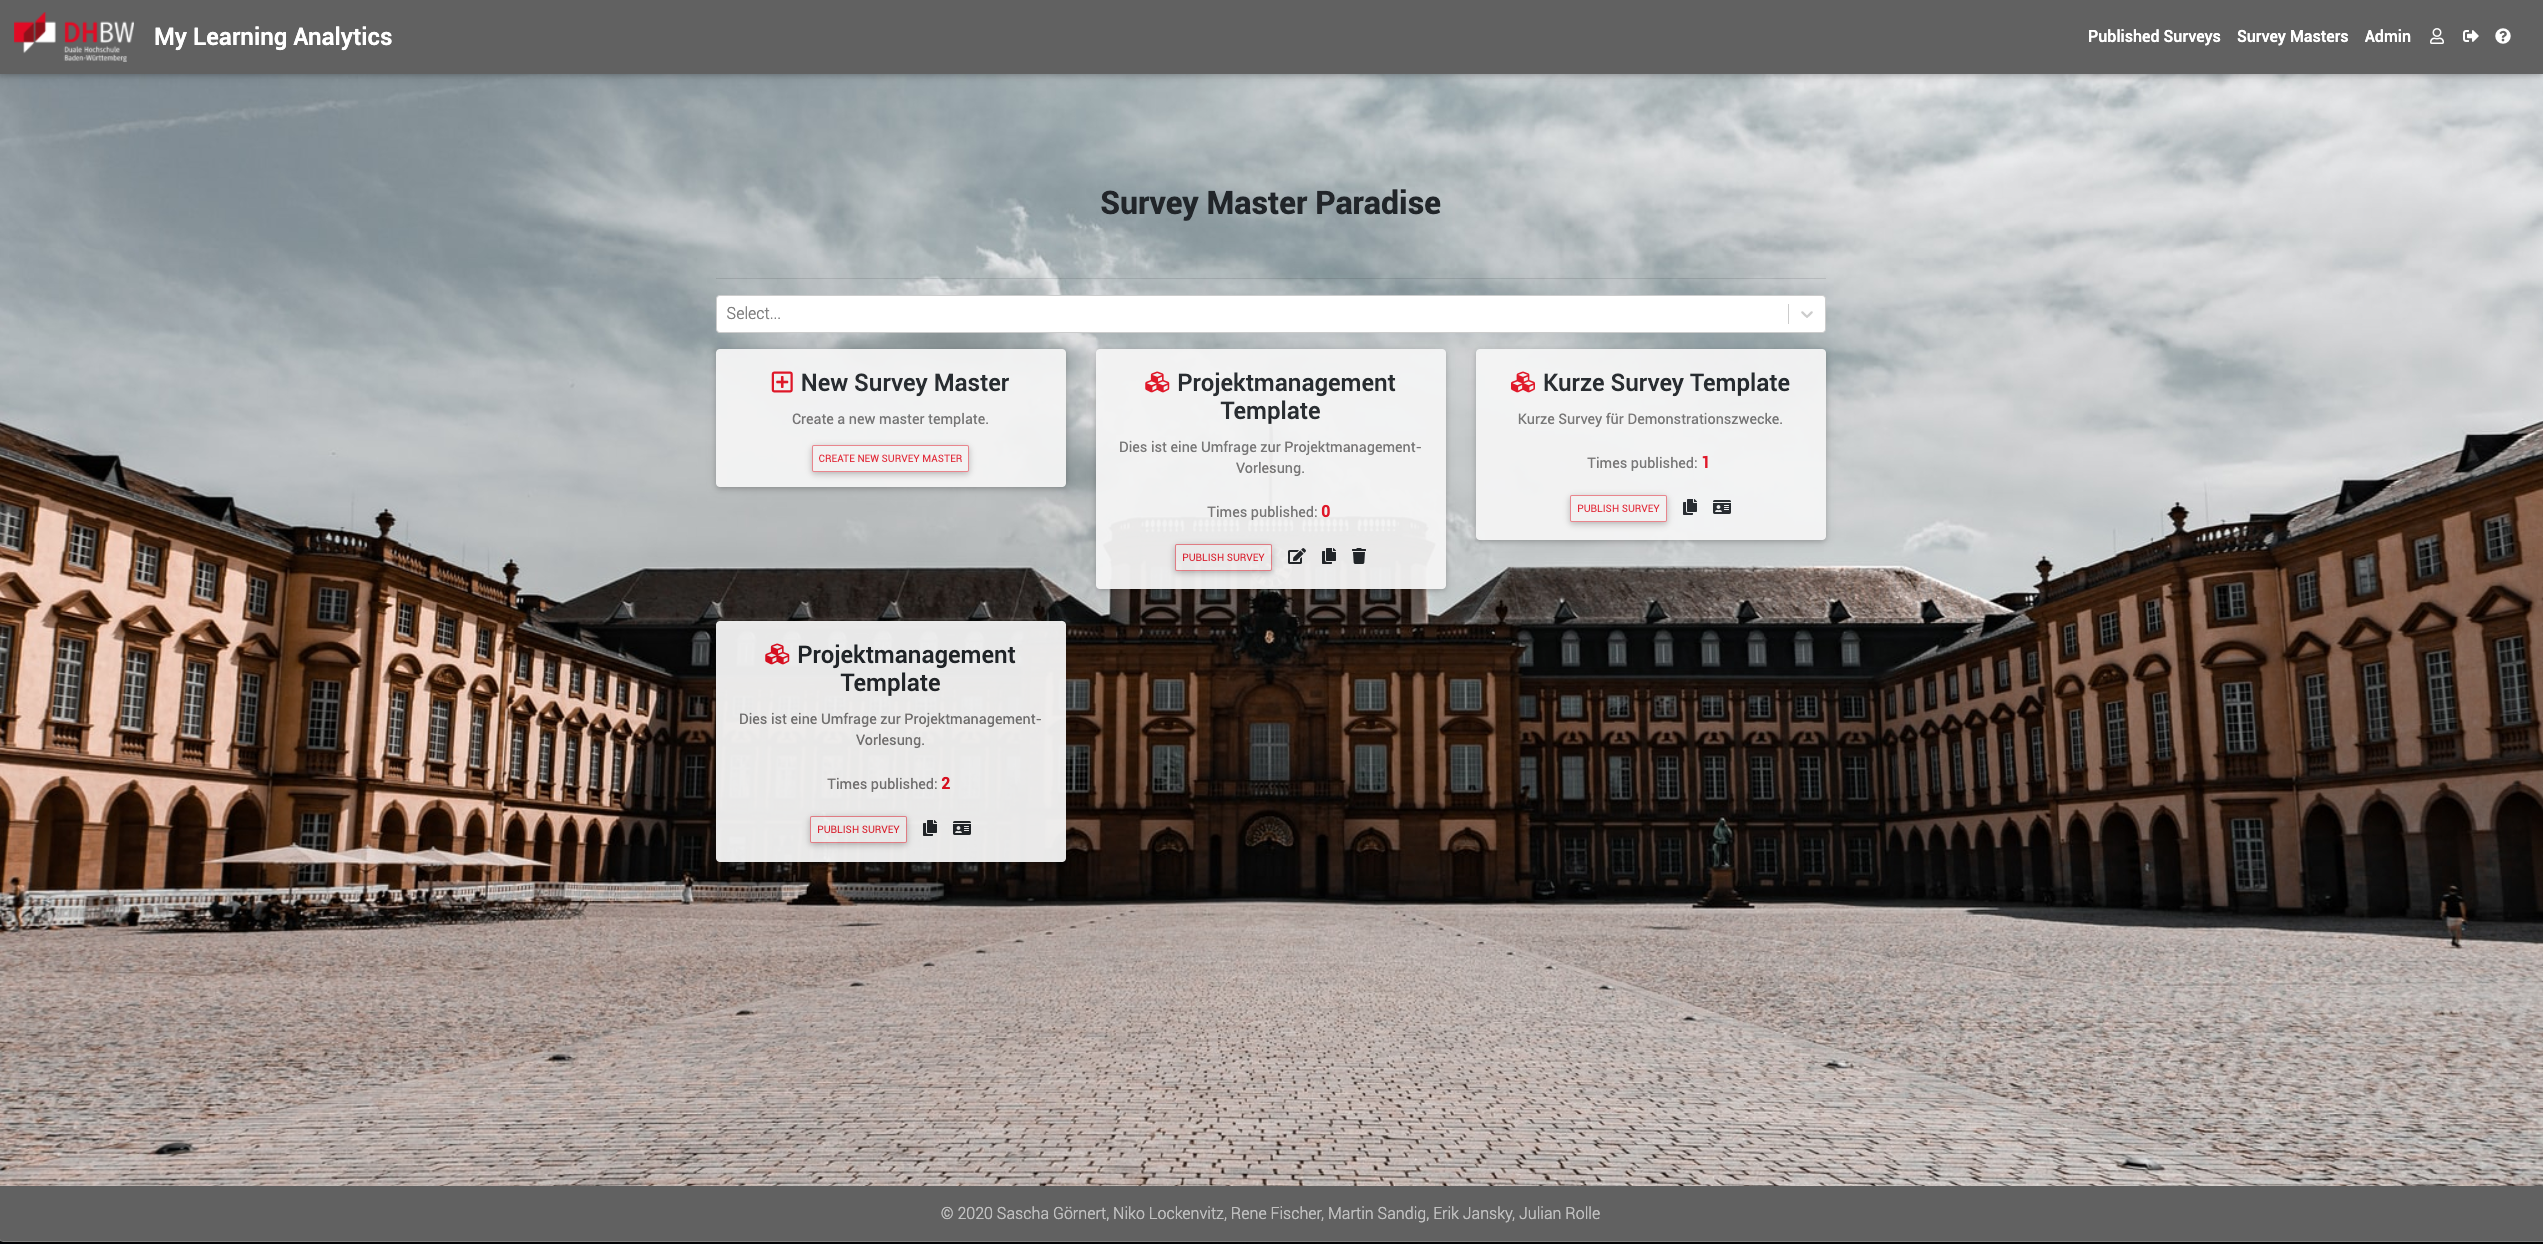
\includegraphics[width=0.95\textwidth, keepaspectratio]{img/client/SurveyMaster.png}
	\captionsetup{justification=centering, format=plain}
	\caption[\acl{UI}: Survey-Dashboard]{\acl{UI}: Survey-Dashboard \\ \quelleScreenshot}
	\label{fig:SurveyMasterDashboard}
\end{figure}
